
%% %%
%% %% INTRO
%% %%


\slide{ A-C ratios: is MET at fault? }
{

\only<1>{
 A/C ratios for data, background-subtracted data, and signal MC. \\
 Looking at MET.
}

\only<7>{
  Conclusions:\\
  \iteb
    \item METMuonBoy closely follows muon $p_T$
    \item A/C disagreements persist even without $MET>25$ and $WMT>40$ cut
    \item Disabling MCP corrections (``C'' term) improves $W^+$ but worsens $W^-$
    \iteb
       \item In any case, these effects are small on the scale of the A/C disagreement
    \itee
  \itee
}

\colb[T]

\column{.5\textwidth}
\centering
\only<2>{ \small{ W: $RefFinal>25$, $W^{+}$}}
\only<3>{ \small{ W: $muPT-MuonBoy$,eta=1.95..2.18,$W^{+}$}}
\only<4>{ \small{ W: $LocHad+muPT>25$,MCP corr,$W^{+}$}}
\only<5>{ \small{ W: $LocHad+muPT>25$,raw muon,$W^{+}$}}
\only<6>{ \small{ W: No MET cut, no WMT cut, $W^{+}$}}
\includegraphics[width=1.0\textwidth]<2>{dates/20130301/figures/AC/W_NOM_Q0_stack_d3_eta_lpt_met_y_2__1_z_0__1_POS}
\includegraphics[width=1.0\textwidth]<3>{dates/20130301/figures/AC/WDB_A_stack_delta_muonboy_muon_POS}
\includegraphics[width=1.0\textwidth]<4>{dates/20130301/figures/AC/WNT_METLOCMUONCORR_Q0_stack_lepton_etav_POS}
\includegraphics[width=1.0\textwidth]<5>{dates/20130301/figures/AC/WNT_METLOCMUON_Q0_stack_lepton_etav_POS}
\includegraphics[width=1.0\textwidth]<6>{dates/20130301/figures/AC/WNT_NOMETMT_Q0_stack_lepton_etav_POS}

\column{.5\textwidth}
\centering
\only<2>{ \small{ W: $RefFinal>25$, $W^{-}$}}
\only<3>{ \small{ W: $muPT-MuonBoy$,eta=1.95..2.18,$W^{-}$}}
\only<4>{ \small{ W: $LocHad+muPT>25$,MCP corr,$W^{-}$}}
\only<5>{ \small{ W: $LocHad+muPT>25$,raw muon,$W^{-}$}}
\only<6>{ \small{ W: No MET cut, no WMT cut, $W^{-}$}}
\includegraphics[width=1.0\textwidth]<2>{dates/20130301/figures/AC/W_NOM_Q0_stack_d3_eta_lpt_met_y_2__1_z_0__1_NEG}
\includegraphics[width=1.0\textwidth]<3>{dates/20130301/figures/AC/WDB_A_stack_delta_muonboy_muon_NEG}
\includegraphics[width=1.0\textwidth]<4>{dates/20130301/figures/AC/WNT_METLOCMUONCORR_Q0_stack_lepton_etav_NEG}
\includegraphics[width=1.0\textwidth]<5>{dates/20130301/figures/AC/WNT_METLOCMUON_Q0_stack_lepton_etav_NEG}
\includegraphics[width=1.0\textwidth]<6>{dates/20130301/figures/AC/WNT_NOMETMT_Q0_stack_lepton_etav_NEG}

\cole
}


\slide{ A-C ratios: W vs Z }
{

\only<1>{
 A/C ratios for data, background-subtracted data, and signal MC. \\
 Comparing with Zs. 
}
\only<5>{
\iteb
\item Recall that the second Z muon is allowed to be ``anywhere''.
\item However, it is in fact highly correlated with the first muon
\iteb
\item E.g., almost always back-to-back in $\phi$.
\itee
\item We can break this correlation by requiring at least one jet.
\iteb
\item The two Z muons would balance agains the jet, and would no longer be back-to-back.
\itee
\itee
}
\only<6>{
\centering
Njets distribution: about 30\% should survive the njet cut \\
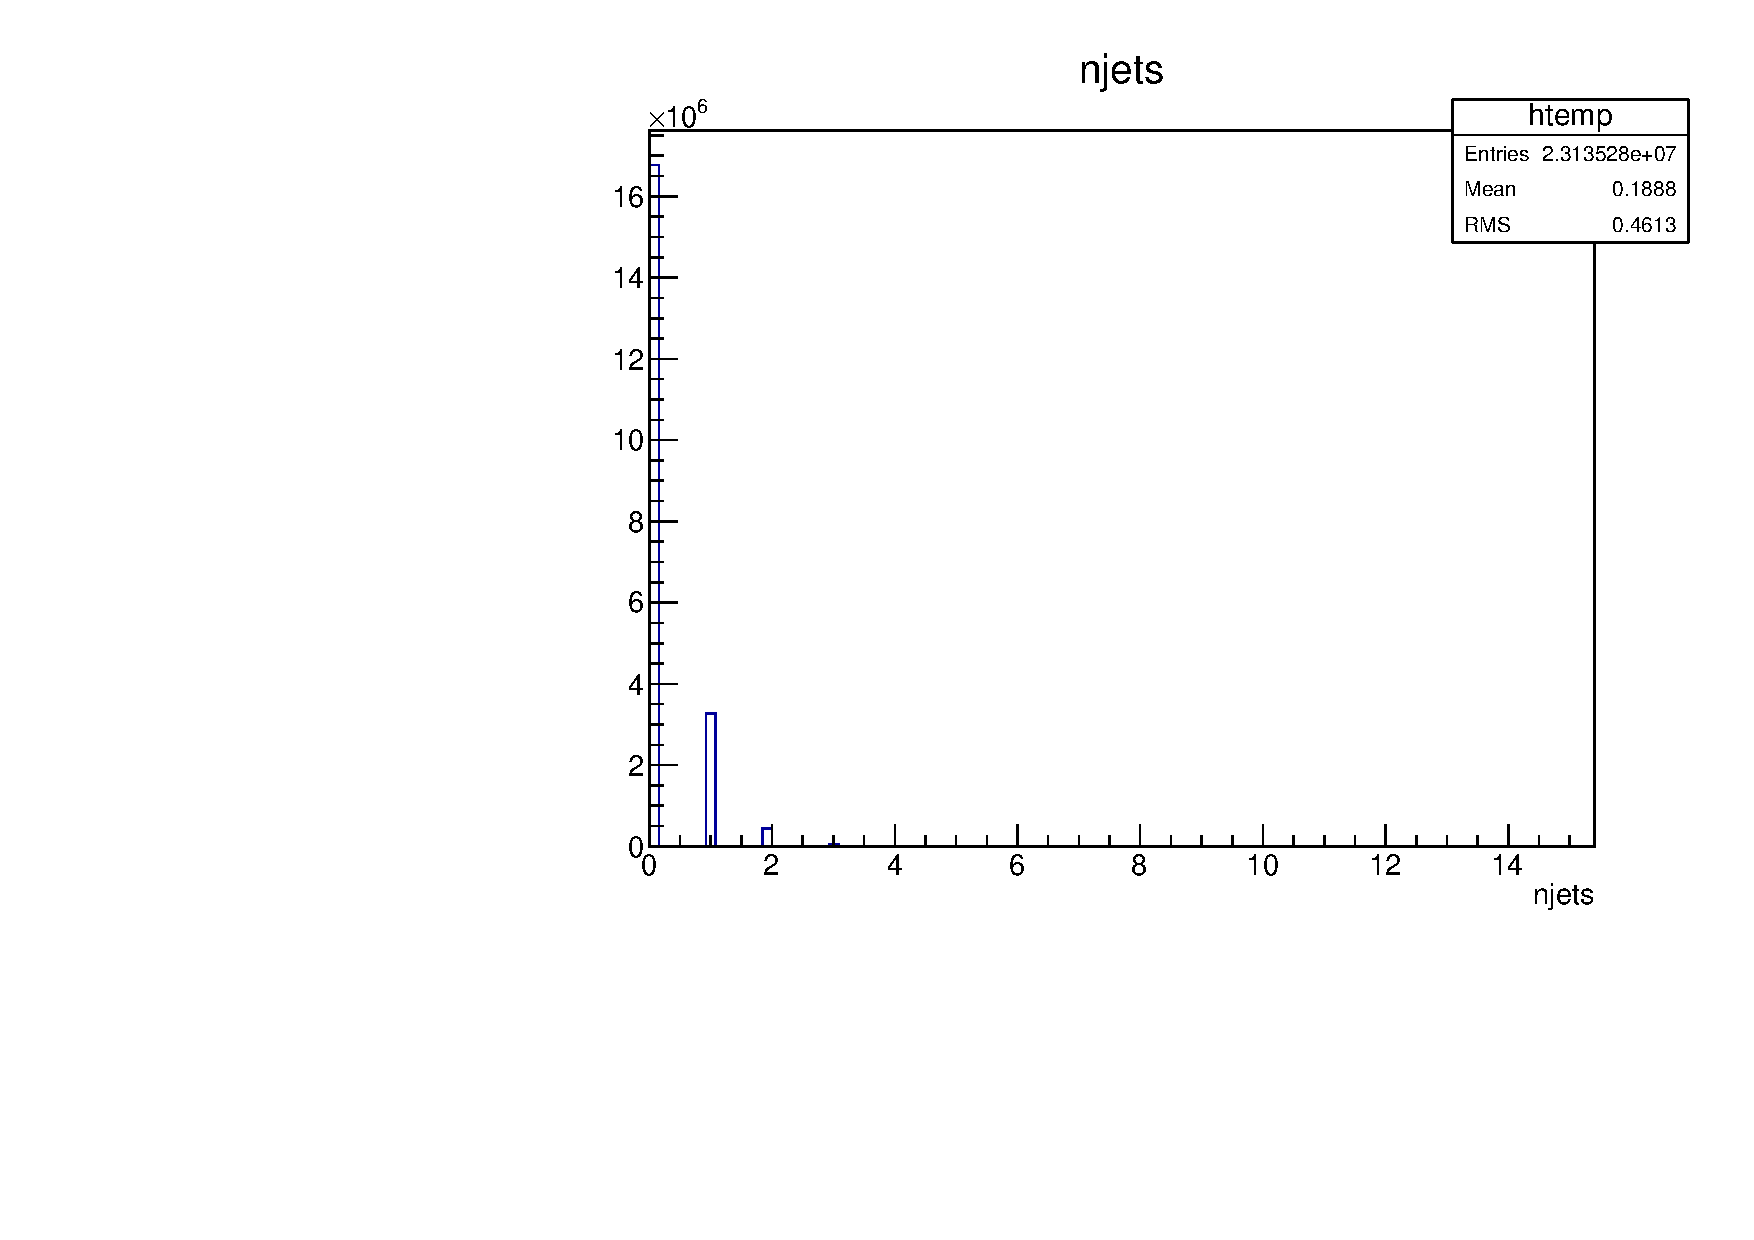
\includegraphics[width=0.6\textwidth]{dates/20130301/figures/njets}
}
\only<9>{
 Conclusions: \\
 \iteb
 \item Statistics in Z+jets events is lower, but there is a hint of similar A/C disagreements seen in Ws.
 \item Could this somehow bias the tag-and-probe scale factors, to the tune of a few percent?
 \itee
}

\colb[T]

\column{.5\textwidth}
\centering
\only<2>{ \small{ $W^{+}$}}
\only<3>{ \small{ Z, no trigger match ($\mu^{+}$)}}
\only<4>{ \small{ Z, trigger match, 2nd muon anywhere ($\mu^{+}$)}}
\only<7>{ \small{ Z, trigger match, $njets>0$ ($\mu^{+}$)}}
\only<8>{ \small{ $W^{+}$ (repeated)}}
\includegraphics[width=1.0\textwidth]<2>{dates/20130301/figures/AC/W_NOM_Q0_stack_d3_eta_lpt_met_y_2__1_z_0__1_POS}
\includegraphics[width=1.0\textwidth]<3>{dates/20130301/figures/AC/ZNT_NOM_stack_leptonP_etav_ALL}
\includegraphics[width=1.0\textwidth]<4>{dates/20130301/figures/AC/ZNT_TMATCHBOTH_stack_leptonP_etav_ALL}
\includegraphics[width=1.0\textwidth]<7>{dates/20130301/figures/AC/ZNT_TMATCHJETS_stack_leptonP_etav_ALL}
\includegraphics[width=1.0\textwidth]<8>{dates/20130301/figures/AC/WNT_NOM_Q0_stack_lepton_etav_POS}

\column{.5\textwidth}
\centering
\only<2>{ \small{ $W^{-}$}}
\only<3>{ \small{ Z, no trigger match ($\mu^{-}$)}}
\only<4>{ \small{ Z, trigger match, 2nd muon anywhere ($\mu^{-}$)}}
\only<7>{ \small{ Z, trigger match, $njets>0$ ($\mu^{-}$)}}
\only<8>{ \small{ $W^{-}$ (repeated)}}
\includegraphics[width=1.0\textwidth]<2>{dates/20130301/figures/AC/W_NOM_Q0_stack_d3_eta_lpt_met_y_2__1_z_0__1_NEG}
\includegraphics[width=1.0\textwidth]<3>{dates/20130301/figures/AC/ZNT_NOM_stack_leptonN_etav_ALL}
\includegraphics[width=1.0\textwidth]<4>{dates/20130301/figures/AC/ZNT_TMATCHBOTH_stack_leptonN_etav_ALL}
\includegraphics[width=1.0\textwidth]<7>{dates/20130301/figures/AC/ZNT_TMATCHJETS_stack_leptonN_etav_ALL}
\includegraphics[width=1.0\textwidth]<8>{dates/20130301/figures/AC/WNT_NOM_Q0_stack_lepton_etav_NEG}

\cole
}



\slide{ A-C ratios: plots in $\phi$ quadrants}
{

\only<1>{
 A/C ratios for data, background-subtracted data, and signal MC. \\
 Here, we are comparing W and Z eta plots in different \red{$\phi$ quadrants}.\\
 \small{Caveat: all scale factors are integrated in $\phi$, so we don't expect excellent agreement here}
}
\only<12>{
 Conclusion: the A-C ratios are very different in the four $\phi$ quadrants. There are substantial detector effects that we don't correct for, and hope they integrate out in $\phi$. \\
 In the barrel, Ws and Zs show similar uncorrected effects. But in forward regions, we see the same W vs Z differences as we saw in phi-integrated plots.
}

\colb[T]

\column{.5\textwidth}
\centering
\only<2>{ \small{ $W^{+}$ (all $\phi$)}}
\only<3>{ \small{ $W^{+}$ ($0 < \phi < PI/2$)}}
\only<4>{ \small{ $W^{+}$ ($PI/2 < \phi < PI$)}}
\only<5>{ \small{ $W^{+}$ ($-PI < \phi < -PI/2$)}}
\only<6>{ \small{ $W^{+}$ ($-PI/2 < \phi < 0$)}}
\only<7>{ \small{ $W^{-}$ (all $\phi$)}}
\only<8>{ \small{ $W^{-}$ ($0 < \phi < PI/2$)}}
\only<9>{ \small{ $W^{-}$ ($PI/2 < \phi < PI$)}}
\only<10>{ \small{ $W^{-}$ ($-PI < \phi < -PI/2$)}}
\only<11>{ \small{ $W^{-}$ ($-PI/2 < \phi < 0$)}}
\includegraphics[width=1.0\textwidth]<2>{dates/20130301/figures/AC/WNT_NOM_Q0_stack_lepton_etav_POS}
\includegraphics[width=1.0\textwidth]<3>{dates/20130301/figures/AC/WNT_NOM_C0_stack_lepton_etav_POS}
\includegraphics[width=1.0\textwidth]<4>{dates/20130301/figures/AC/WNT_NOM_C1_stack_lepton_etav_POS}
\includegraphics[width=1.0\textwidth]<5>{dates/20130301/figures/AC/WNT_NOM_C2_stack_lepton_etav_POS}
\includegraphics[width=1.0\textwidth]<6>{dates/20130301/figures/AC/WNT_NOM_C3_stack_lepton_etav_POS}
\includegraphics[width=1.0\textwidth]<7>{dates/20130301/figures/AC/WNT_NOM_Q0_stack_lepton_etav_NEG}
\includegraphics[width=1.0\textwidth]<8>{dates/20130301/figures/AC/WNT_NOM_C0_stack_lepton_etav_NEG}
\includegraphics[width=1.0\textwidth]<9>{dates/20130301/figures/AC/WNT_NOM_C1_stack_lepton_etav_NEG}
\includegraphics[width=1.0\textwidth]<10>{dates/20130301/figures/AC/WNT_NOM_C2_stack_lepton_etav_NEG}
\includegraphics[width=1.0\textwidth]<11>{dates/20130301/figures/AC/WNT_NOM_C3_stack_lepton_etav_NEG}

\column{.5\textwidth}
\centering
\only<2>{ \small{ $Z^{+}$ (all $\phi$)}}
\only<3>{ \small{ $Z^{+}$ ($0 < \phi < PI/2$)}}
\only<4>{ \small{ $Z^{+}$ ($PI/2 < \phi < PI$)}}
\only<5>{ \small{ $Z^{+}$ ($-PI < \phi < -PI/2$)}}
\only<6>{ \small{ $Z^{+}$ ($-PI/2 < \phi < 0$)}}
\only<7>{ \small{ $Z^{-}$ (all $\phi$)}}
\only<8>{ \small{ $Z^{-}$ ($0 < \phi < PI/2$)}}
\only<9>{ \small{ $Z^{-}$ ($PI/2 < \phi < PI$)}}
\only<10>{ \small{ $Z^{-}$ ($-PI < \phi < -PI/2$)}}
\only<11>{ \small{ $Z^{-}$ ($-PI/2 < \phi < 0$)}}
\includegraphics[width=1.0\textwidth]<2>{dates/20130301/figures/AC/ZNT_TMATCHBOTH_stack_leptonP_etav_ALL}
\includegraphics[width=1.0\textwidth]<3>{dates/20130301/figures/AC/ZNT_TB_C0_stack_leptonP_etav_ALL}
\includegraphics[width=1.0\textwidth]<4>{dates/20130301/figures/AC/ZNT_TB_C1_stack_leptonP_etav_ALL}
\includegraphics[width=1.0\textwidth]<5>{dates/20130301/figures/AC/ZNT_TB_C2_stack_leptonP_etav_ALL}
\includegraphics[width=1.0\textwidth]<6>{dates/20130301/figures/AC/ZNT_TB_C3_stack_leptonP_etav_ALL}
\includegraphics[width=1.0\textwidth]<7>{dates/20130301/figures/AC/ZNT_TMATCHBOTH_stack_leptonN_etav_ALL}
\includegraphics[width=1.0\textwidth]<8>{dates/20130301/figures/AC/ZNT_TB_C0_stack_leptonN_etav_ALL}
\includegraphics[width=1.0\textwidth]<9>{dates/20130301/figures/AC/ZNT_TB_C1_stack_leptonN_etav_ALL}
\includegraphics[width=1.0\textwidth]<10>{dates/20130301/figures/AC/ZNT_TB_C2_stack_leptonN_etav_ALL}
\includegraphics[width=1.0\textwidth]<11>{dates/20130301/figures/AC/ZNT_TB_C3_stack_leptonN_etav_ALL}

\cole
}



\slide{ Inside the $|\eta|=1.95-2.18$ bin}
{

\only<1>{
 $\eta$ and $\phi$ distributions inside one of the worst eta bins. \\
 \small{Caveat: all scale factors are integrated in $\phi$, so we don't expect excellent agreement here}
}

\only<10>{
W and Z side-by-side:
}

\only<15>{
 Conclusions: \\
 \iteb
 \item Strange structure seen both in $\phi$ and $\eta$ within $|\eta|=1.95-2.18$ slice
 \item Some of it is similar in W and Z events, but some it \red{not}.
 \item Also, it is somewhat charge-dependent
 \itee
} 

\colb[T]

\column{.5\textwidth}
\centering
\only<2>{ \small{ A-side $W^{+}$ ($\eta$)}}
\only<3>{ \small{ A-side $W^{-}$ ($\eta$)}}
\only<4>{ \small{ A-side $W^{+}$ ($\phi$)}}
\only<5>{ \small{ A-side $W^{-}$ ($\phi$)}}
\only<6>{ \small{ A-side $Z^{+}$ ($\eta$)}}
\only<7>{ \small{ A-side $Z^{-}$ ($\eta$)}}
\only<8>{ \small{ A-side $Z^{+}$ ($\phi$)}}
\only<9>{ \small{ A-side $Z^{-}$ ($\phi$)}}
\only<11>{ \small{ A-side $W^{-}$ ($\eta$)}}
\only<12>{ \small{ A-side $W^{-}$ ($\phi$)}}
\only<13>{ \small{ C-side $W^{-}$ ($\eta$)}}
\only<14>{ \small{ C-side $W^{-}$ ($\phi$)}}
\includegraphics[width=1.0\textwidth]<2>{dates/20130301/figures/AC/WDB_A_stack_l_eta_POS}
\includegraphics[width=1.0\textwidth]<3>{dates/20130301/figures/AC/WDB_A_stack_l_eta_NEG}
\includegraphics[width=1.0\textwidth]<4>{dates/20130301/figures/AC/WDB_A_stack_l_phi_POS}
\includegraphics[width=1.0\textwidth]<5>{dates/20130301/figures/AC/WDB_A_stack_l_phi_NEG}
\includegraphics[width=1.0\textwidth]<6>{dates/20130301/figures/AC/ZDB_A_stack_lP_eta_ALL}
\includegraphics[width=1.0\textwidth]<7>{dates/20130301/figures/AC/ZDB_A_stack_lN_eta_ALL}
\includegraphics[width=1.0\textwidth]<8>{dates/20130301/figures/AC/ZDB_A_stack_lP_phi_ALL}
\includegraphics[width=1.0\textwidth]<9>{dates/20130301/figures/AC/ZDB_A_stack_lN_phi_ALL}
\includegraphics[width=1.0\textwidth]<11>{dates/20130301/figures/AC/WDB_A_stack_l_eta_NEG}
\includegraphics[width=1.0\textwidth]<12>{dates/20130301/figures/AC/WDB_A_stack_l_phi_NEG}
\includegraphics[width=1.0\textwidth]<13>{dates/20130301/figures/AC/WDB_C_stack_l_eta_NEG}
\includegraphics[width=1.0\textwidth]<14>{dates/20130301/figures/AC/WDB_C_stack_l_phi_NEG}

\column{.5\textwidth}
\centering
\only<2>{ \small{ C-side $W^{+}$ ($\eta$)}}
\only<3>{ \small{ C-side $W^{-}$ ($\eta$)}}
\only<4>{ \small{ C-side $W^{+}$ ($\phi$)}}
\only<5>{ \small{ C-side $W^{-}$ ($\phi$)}}
\only<6>{ \small{ C-side $Z^{+}$ ($\eta$)}}
\only<7>{ \small{ C-side $Z^{-}$ ($\eta$)}}
\only<8>{ \small{ C-side $Z^{+}$ ($\phi$)}}
\only<9>{ \small{ C-side $Z^{-}$ ($\phi$)}}
\only<11>{ \small{ A-side $Z^{-}$ ($\eta$)}}
\only<12>{ \small{ A-side $Z^{-}$ ($\phi$)}}
\only<13>{ \small{ C-side $Z^{-}$ ($\eta$)}}
\only<14>{ \small{ C-side $Z^{-}$ ($\phi$)}}
\includegraphics[width=1.0\textwidth]<2>{dates/20130301/figures/AC/WDB_C_stack_l_eta_POS}
\includegraphics[width=1.0\textwidth]<3>{dates/20130301/figures/AC/WDB_C_stack_l_eta_NEG}
\includegraphics[width=1.0\textwidth]<4>{dates/20130301/figures/AC/WDB_C_stack_l_phi_POS}
\includegraphics[width=1.0\textwidth]<5>{dates/20130301/figures/AC/WDB_C_stack_l_phi_NEG}
\includegraphics[width=1.0\textwidth]<6>{dates/20130301/figures/AC/ZDB_C_stack_lP_eta_ALL}
\includegraphics[width=1.0\textwidth]<7>{dates/20130301/figures/AC/ZDB_C_stack_lN_eta_ALL}
\includegraphics[width=1.0\textwidth]<8>{dates/20130301/figures/AC/ZDB_C_stack_lP_phi_ALL}
\includegraphics[width=1.0\textwidth]<9>{dates/20130301/figures/AC/ZDB_C_stack_lN_phi_ALL}
\includegraphics[width=1.0\textwidth]<11>{dates/20130301/figures/AC/ZDB_A_stack_lN_eta_ALL}
\includegraphics[width=1.0\textwidth]<12>{dates/20130301/figures/AC/ZDB_A_stack_lN_phi_ALL}
\includegraphics[width=1.0\textwidth]<13>{dates/20130301/figures/AC/ZDB_C_stack_lN_eta_ALL}
\includegraphics[width=1.0\textwidth]<14>{dates/20130301/figures/AC/ZDB_C_stack_lN_phi_ALL}

\cole
}


%%%%%%% Back-up slides %%%%%%%%%%
\appendix
\newcounter{finalframe}
\setcounter{finalframe}{\value{framenumber}}

\slide{}
{

\centering
\Huge Back-up slides
}



\slide{Conclusions}
{
\centering
Hm
}
